%Latex Template (Master file): Updated  11 April 2024
% Two side printing enabled
% By Sanjay S. Shitole : modified on 28 feb 2011.
% Pl. note : this template is used for practice and to show the different functions of LaTeX. Refered citations are not actuals.
%-------------------------------------------------------------
%--------------------------------------------------------------
%Pl. refer the  database.bib file in the folder for references list
% study the syntax for refernces as shown in database.bib

%--------------------------------------------------------
%--------------------------------------------------------
% To create list of table  --
% Run the code twice (pdflatex or latex)
%%%%%%%%%%%%%%%%%%%%%%%%%%%%%%%%%%%%
%To get the references using bibtex follow following sequence.
%pdflatex
%bibtex
%pdflatex
%pdflatex
%%%%%%%%%%%%%%%%%%%%%%%%%%%%%%%%%%%%%%%%%%%%%%%%%%%%%
%%%%%%%%%%%%%%%%%%%%%%%%%%%%%%%%%%%%%%%%%%%%%%%%%%%
\documentclass[11pt,a4paper,final,twoside]{report}

\usepackage{geometry}
\usepackage{amsfonts}
\usepackage{amssymb}
\usepackage{graphics}
\usepackage{graphicx}
\usepackage{amsmath}
\usepackage{array}
\usepackage[pdftex]{hyperref}
\usepackage{epstopdf}
\usepackage{setspace}
\usepackage{natbib}


\begin{document}

\thispagestyle{empty}
%%%% This is first page
%%%%% Refer q31.tex file

\begin{center}
A Project Report On

\LARGE{Topic Name}

\end{center}

\vspace{3cm}

\begin{center}

Submitted in partial fulfilment for the
\linebreak degree of Bachelor of Technology in 
\linebreak  --------(Dept Name)
\end{center}
\vspace{2cm}
\begin{center}

Submitted by
\linebreak \textbf{Name of Student (Roll No)}
\linebreak \textbf{Name of Student (Roll No)}
\linebreak \textbf{Name of Student (Roll No)}

\vspace{0.5cm}

 Under the guidance of
\linebreak \textbf{Guide Name}
\end{center} 

\vspace{1cm}
\begin{center}

\vspace{0.5cm}
 


\vspace{0.1cm}
\begin{figure}[!h]
	\begin{center}
		
\includegraphics[width=4cm,height=4cm,keepaspectratio]{SNDT_logo.pdf}
	\end{center}
	%\caption{}
\end{figure}
\vspace{0.1cm}

 \textbf{Name of College}
\linebreak Address 
\linebreak Address
\linebreak Year
\end{center}


%\end{document}

\begin{center}
	\textbf{\Large Declaration}
\end{center}

I, \textbf{[Your Full Name]}, hereby declare that the work presented in this \textit{project} entitled ``\textit{[Title of Your Work]}'' is entirely my own. The content of this \textit{ project} has been generated through my independent efforts, research, and scholarly contributions. I further declare that:
\begin{enumerate}
	\item \textbf{Originality:}
	\begin{itemize}
		\item The ideas, concepts, and contributions presented in this work are solely the result of my own intellectual endeavours.
	\end{itemize}
		\item \textbf{Authenticity:}
	\begin{itemize}
		\item All data, figures, tables, and findings presented in this \textit{project}are genuine and have not been fabricated or manipulated.
	\end{itemize}
		\item \textbf{No Use of AI Tools:}
	\begin{itemize}
		\item I have not used any AI-based tools to generate significant portions of this \textit{ project} including but not limited to content, research objectives, hypotheses, and analysis.
	\end{itemize}
		\item \textbf{No Plagiarism:}
	\begin{itemize}
		\item I have properly cited and referenced all external sources and works consulted during the preparation of this \textit{[thesis/dissertation/research project]}.
		\item There is no instance of plagiarism or unauthorized use of others' intellectual property.
	\end{itemize}
		\item \textbf{Independent Work:}
	\begin{itemize}
		\item This work has been conducted independently, without any collaboration or assistance that would compromise the originality of the content.
	\end{itemize}
		\item \textbf{Academic Integrity:}
	\begin{itemize}
		\item I have adhered to the principles of academic integrity and ethical research throughout the entire process of producing this \textit{[thesis/dissertation/research project]}.
	\end{itemize}
\end{enumerate}
I understand the consequences of academic dishonesty and affirm that this declaration accurately reflects the nature and authenticity of my work.
\begin{flushright}
	\textbf{Date:} \textit{[Date of Submission]}
\end{flushright}
\begin{flushright}
	\textbf{Signature:} \underline{\hspace{5cm}} \\
	\textit{[Your Full Name]}
\end{flushright}
%%%%%%%%%%%%%% this is for certificate, pl modify according to your need
% refer q31.tex

\newpage
\thispagestyle{empty}
\begin{center}
\LARGE{CERTIFICATE}
\end{center}


\vspace{2cm}

This is to certify that  (---Name of student) has completed the -----
(project-I/ Project-II..etc as per structure  of syllabus)
 report on the topic `` topic name '' satisfactorily in partial fulfillment for the Bachelor's Degree in --------(dept) under the guidance of ----Guide Name during the year ----- as prescribed by ---- Shreemati Nathibai Damodar Thackersey Women's University (SNDTWU) 
\vspace{3cm}

\begin{flushleft}
Guide \hspace{95.00mm} Head of Department\newline



Guide name \hspace{80.00mm}    HOD name
\end{flushleft}



\vspace{2cm}
\begin{center}
Principal



Name of Principal
\end{center}

\vspace{2cm}
\begin{flushleft}
Examiner 1 \hspace{100.00mm} Examiner 2
\end{flushleft}

\newpage





\pagenumbering{roman}
%%%%%%%%%%%%%%%%%%% use for abstract
%%% refer q31.tex
\begin{abstract}
	This abstract provides a concise summary of the main points and findings of your research paper, thesis, or article. It should be clear, informative, and engaging, allowing readers to quickly understand the purpose and significance of your work.
	
	\textbf{Introduction:} Start by introducing the topic and providing context for your study.
	
	\textbf{Objective/Research Question:} State the main objective of your research or the specific research question you aimed to address.
	
	\textbf{Methodology:} Briefly describe the methods or approaches used to conduct your research. This may include experimental techniques, data collection methods, or theoretical frameworks.
	
	\textbf{Results/Findings:} Summarize the main findings or outcomes of your study. Highlight the key results that contribute to addressing your research question.
	
	\textbf{Conclusion/Implications:} Conclude with the significance of your findings and discuss any potential implications or applications of your research.
	
	This abstract should be concise, typically between 150-250 words, and written in clear, direct language. Avoid unnecessary jargon or complex terminology.
	
	Keywords: Include relevant keywords that reflect the main topics and themes of your research. This helps with indexing and searchability.
\end{abstract}


  \addcontentsline{toc}{chapter}{Abstract}
%\clearpage
\tableofcontents
  
\listoftables
   \addcontentsline{toc}{chapter}{List of Tables}


\listoffigures
  \addcontentsline{toc}{chapter}{List of Figures}

%\def\abstract{
 % \chapter*{Abstract}
  %\addcontentsline{toc}{chapter}{Abstract}
  %\relax\markboth{ABSTRACT}{ABSTRACT}}
%\def\endabstract{\par\newpage}


%%% refer q31.tex 


% NOMENCLATURE
%\newpage
\chapter*{Nomenclature}
%\begin{flushleft}
%\textbf{\begin{LARGE}
%Nomenclature
%\end{LARGE}}
%\end{flushleft}
%
%\vspace{0.3in}

\begin{description}
\item{\makebox[0.75in][l]{$ dB  $}}  Decibel
\item{\makebox[0.75in][l]{$ \sigma_{s} $}} 3 dB Bandwidth of source
\item{\makebox[0.75in][l]{3G}} Third generation
\item{\makebox[0.75in][l]{4G}} Fourth Generation
\item{\makebox[0.75in][l]{TDM}} Time Division Multiplexing
\item{\makebox[0.75in][l]{WDM}} Wavelength Division Multiplexing
\end{description}

\addcontentsline{toc}{chapter}{Nomenclature}


\newpage

\pagestyle{plain}
\pagenumbering{arabic}
%\singlespacing
\onehalfspacing
%\doublespacing

%% refer q31.tex

	\chapter{Introduction}
	
	% Introduction content goes here
	This chapter serves as the introduction to the document. It provides an overview of the topic, establishes the context and significance of the research, and outlines the objectives and scope of the study.
	
	\section{Background}
	% Background information and context
	Provide background information on the topic of the study. Discuss relevant literature, previous research, and key concepts related to the subject matter.
	
	\section{Research Motivation}
	% Motivation for the research
	Explain the motivation behind conducting this research. Describe why the topic is important and relevant, highlighting any gaps or challenges that the study aims to address.
	
	\section{Research Objectives}
	% Objectives of the research
	Outline the specific objectives and goals of the research. Clearly state what the study aims to achieve and the questions it seeks to answer.
	
	\section{Scope of the Study}
	% Scope of the research
	Define the scope of the study by specifying the boundaries and limitations. Describe what aspects will be included and excluded from the investigation.
	
	\section{Structure of the Document}
	% Structure of the document
	Provide an overview of the document's structure. Briefly outline the chapters or sections that follow and explain how they contribute to addressing the research objectives.
	


%% refer q31.tex

\chapter{Review of Literature }
This chapter should consists the information regarding already available solutions/methods of whatever you are proposing. 

	
	\section*{Introduction}
	Provide an introduction to the literature review, explaining the importance of the topic and the objectives of the review.
	
	\section*{Scope and Objectives}
	Define the scope of the literature review and outline the specific objectives.
	
	\section*{Methodology}
	Describe the methodology used for literature search and selection of sources.
	
	\section*{Review of Literature}
	
	% Example of Including Citations and Summaries
	\subsection*{Theme 1: [Title of Theme]}
	\begin{itemize}
		\item \citet{author1_year}: Summary of key findings and methodologies.
		\item \citet{author2_year}: Comparison with previous studies and critical analysis.
	\end{itemize}
	
	\subsection*{Theme 2: [Title of Theme]}
	\begin{itemize}
		\item \citet{author3_year}: Discussion of trends and gaps in the literature.
		\item \citet{author4_year}: Analysis of conflicting viewpoints and implications.
	\end{itemize}
	
	\section*{Synthesis and Discussion}
	Synthesize the findings from different sources and discuss their implications for your research question.
	
	\section*{Conclusion}
	Summarize the main findings of the literature review and highlight areas for further research.
	




\chapter{Methodology / Research Methodology/ Experimental Methodology / Analytical Methodology/Descriptive Methodology /Case Study Methodology  / Quantitative Research Methodology}


Select any suitable title fro this topic based on your project
	
	\section{Introduction to Methodology}
	\textbf{Purpose:} The objective of the Methodology chapter is to describe the research approach and methods used to address the project objectives.
	
	\textbf{Context:} This section provides a brief overview of the project and explains its significance in the context of the field of study.
	
	\section{Research Design}
	\textbf{Describe Research Design:} The overall research design adopted for the project is \textit{[insert type of research design]} (e.g., experimental, analytical, descriptive, case study).
	
	\textbf{Justification:} This research design was chosen because \textit{[provide reasons why this design aligns with the project goals]}.
	
	\section{Research Approach}
	\textbf{Explain Approach:} The approach used to collect data or information is \textit{[insert type of research approach]} (e.g., quantitative, qualitative, mixed-methods).
	
	\textbf{Rationale:} This approach was selected based on \textit{[explain how it aligns with the research questions and objectives]}.
	
	\section{Sampling Strategy}
	\textbf{Define Sampling:} The sampling technique used is \textit{[describe sampling technique]} (e.g., random sampling, purposive sampling).
	
	\textbf{Sample Size:} The sample size of \textit{[specify sample size]} was chosen to \textit{[justify representativeness or reliability]}.
	
	\section{Data Collection Methods}
	\textbf{Detail Data Collection:} Data was gathered using \textit{[describe data collection methods]} (e.g., surveys, interviews, experiments, observations).
	
	\textbf{Instruments Used:} The tools and instruments utilized include \textit{[mention specific tools or technologies]}.
	
	\section{Data Analysis Techniques}
	\textbf{Outline Analysis Methods:} Collected data will be analyzed using \textit{[explain analysis methods]} (e.g., statistical analysis, thematic analysis, content analysis).
	
	\textbf{Software Tools:} Analysis will be conducted using \textit{[mention software tools or packages]} (e.g., SPSS, MATLAB, NVivo).
	
	\section{Research Ethics}
	\textbf{Ethical Considerations:} Ethical issues related to data collection, participant consent, and confidentiality were addressed by \textit{[explain ethical considerations]}.
	
	\textbf{Compliance:} The research adheres to ethical guidelines and regulations set by \textit{[mention relevant regulatory bodies]}.
	
	\section{Limitations and Assumptions}
	\textbf{Identify Limitations:} Potential limitations in the research approach or methods include \textit{[acknowledge limitations]}.
	
	\textbf{Discuss Assumptions:} Assumptions made during the research process are \textit{[state assumptions]}.
	
	\section{Validation and Reliability}
	\textbf{Ensure Validity:} Steps taken to ensure validity and reliability include \textit{[describe validation methods]} (e.g., triangulation, pilot testing).
	
	\section{Timeline and Schedule}
	\textbf{Project Timeline:} A brief timeline outlining the sequence of research activities and milestones is provided in \textit{[include project timeline]}.
	
	\textbf{Gantt Chart (Optional):} A Gantt chart or schedule diagram can be included to visualize the project timeline.
	
	\section{Writing Tips}
	\begin{itemize}
		\item Use clear and concise language to describe each methodological aspect.
		\item Provide sufficient detail for readers to understand the research process and its rationale.
		\item Include citations to relevant sources to support methodological choices.
		\item Organize the chapter logically, following a structured format from general to specific details.
	\end{itemize}
	





%%%%%%%%%%%%%%%%%%%%%%%%%%%%%%%%%%%%%%%%%%%%%%%%%%%%%%%%
%%%%% for Quick help  folloowng lien are useful
%%%%%%%%%%%%%%%%%%%%%%%%%%%%%%%%%%%%%%

Study the \LaTeX\ code in chapt3.tex.
It will help you for figure insertion, math using \LaTeX\ .\, Table creation,
citations, labels.
\section{Homomorphic filter} 
 %Morphological filters
By performing simultaneous gray level range compression and contrast enhancement on illumination reflection model,one can improve the appearance of an image by designing a frequency domain procedure~\cite{man87}.
An image $f(x,y)$ can be expressed as a product of illumination and reflection components~\cite{sam09}.

 % NOTE2: pl.refer that  $ $ sign for mathamatical term in the text in line.

\begin{equation}
f(x,y)=i(x,y)r(x,y)
\end{equation}

% NOTE3:- \[ f(x,y)=i(x,y)r(x,y) \]
% this has the same effect as above code i.e
%  \begin{equation}
% f(x,y)=i(x,y)r(x,y)
% \end{equation}

here $ i(x,y) $ is  illumination component and  $ r(x,y) $ reflection component.\\

% NOTE 4: Observe the  \\  at the end
% this will help the latex to go to new line.


Fourier transform of the product of two functions is not separable, So we can define shown in as shown in Equation~\ref{fourier}

\begin{equation}
F.T[z(x,y)]=F.T[ln f(x,y)]=F.T[ln i(x,y)]+F.T[ln r(x,y)]
\label{fourier}
\end{equation}

\begin{equation}
Z(u,v)=F_{i}(u,v)+F_{r}(u,v)
\end{equation}


 \begin{equation}
  S(u,v)=H(u,v)Z(u,v)
 \end{equation}

% Note5: Observe the following code ,
% here for the equatins \[                      \] brackets are used
% this will help you if you are not interested in numbering of the equations.
% observe the effect in output pdf file.


 where $S(u,v)$ Fourier Transform of result  and $H(u,v)$ Filter function

      \[S(u,v)=H(u,v)F_{i}(u,v)+H(u,v)F_{r}(u,v)\]

      \[s(x,y)=F^{-1}[S(u,v)]\]

      \[s(x,y)=F^{-1}[H(u,v)F_{i}(u,v)]+F^{-1}[H(u,v)F^{r}(u,v)]\]

      Say
      \[i'(x,y)=F^{-1}[H(u,v)F_{i}(u,v)]\]

       \[r'(x,y)=F^{-1}[H(u,v)F_{r}(u,v)]\]

       Hence,
       \[s(x,y)=i'(x,y)+r'(x,y)\]

       Therefore,
       Let $g(x,y)$ be the inverse exponential operation

       \[g(x,y)=e^{s(x,y)}\]

      \[g(x,y)=e^{i'(x,y)}e^{r'(x,y)}\]

       \[g(x,y)=i_{0}(x,y)+r_{0}(x,y)\]

       where $i_{0}(x,y)=e^{i'(x,y)}$ and $r_{0}(x,y)=e^{r'(x,y)}$


%  Note 6:following five lines are responsible for graphics insertion.

\begin{figure}[h]
	\centering
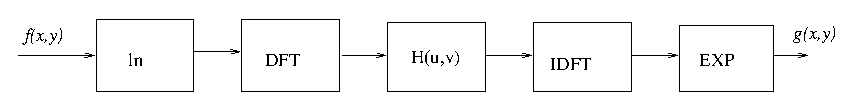
\includegraphics{blockdig.eps}
\caption{Block digram}
	\label{bbb}
\end{figure}

\begin{itemize}
\item This approach is used for homomorphic filtering as shown in figure~\ref{bbb}. The key to the approach is separation of the illumination and reflection components. Between them $i(x,y)$ contributes to the low frequency since illumination is more or less uniform and $r(x,y)$ is high frequency component as it tends to vary abruptly at junctions of dissimilar objects.
\item $H(u,v)$ is the homomorphic filtering function.A typical homomorphic filter $H(u,v)$ is as shown in figure below. Generally, $\gamma_L<1$ and$\gamma_H>1$, $H(u,v)$ tends to decrease the contribution made by low frequencies and amplify the contribution made by high frequency.
\end{itemize}

%NOTE 7: The following five lines are responsible for graphics insertion.
% Also note that in caption q312 is the figure number and after : put name of the figure.

\begin{figure}[htbp]
\centering
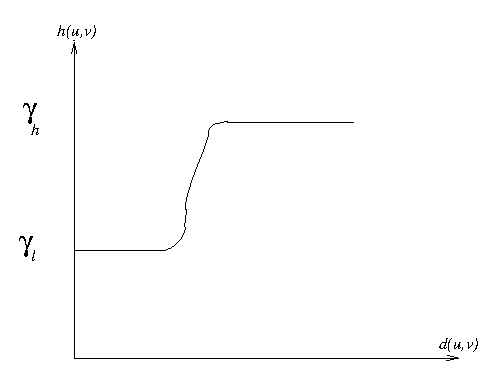
\includegraphics{graph.eps}
\caption{Transfer function}
\label{fig:graph}
\end{figure}

\section{Morphological Filters}

To understand morphological filters we first need to understand the operations dilation, erosion,opening  and  closing.

\subsection{Dilation}
With $A$ and $B$ as sets in $Z^{2}$,the dilation of $A$ and $B$ denoted as $A\oplus B$ is defined as

\[A\oplus B={Z/(\hat{B}_{z}\cap A \neq \phi}\]

Equation obtained by reflection of $B$ about origin and shifting reflection by $ z$ .
$B$  and $A$ should overlap by at least one element.Set $B$ is the structuring element in all morphological operations.\\
 \textbf{Erosion} For sets $A$ and $B$ in $Z^{2}$,the erosion of $A$ by $B$ denoted as $A\ominus B$ is defined as

\[ A\ominus B={Z/(B_{z}\subseteq A )} \]
This equation indicates that the erosion of $A$ by $B$ is the set of all points $z$ such that $B$,translated by $z$ is contained in $A$ Erosion shrinks an image.

\subsection{Opening and closing}

Opening smooths the contour of an object.
 Closing also tends to smooth sections of contours but it generally fuses narrow breaks and long thin gulfs,eliminates small holes and fills gaps in contour.
Opening is denoted by $A\circ B$

\[A\circ B=(A\ominus B)\oplus B\]

  i.e. Erosion followed by dilation
 Closing is denoted by $A\bullet B$

 \[A\bullet B=(A\oplus B)\ominus B\]

 i.e Dilation followed by erosion.
 Morphological operations can be used to construct filters.

\begin{enumerate}
	\item Suppose we have a binary image which is corrupted by noise.The noise manifests itself as light elements on a dark background and dark elements on  light components of image .
	\item A morphological filter consisting of opening followed by closing operation eliminates the noise and its effect on the image while distorting it as little as possible.
	\item The steps are as follows

\begin{itemize}
	\item We have a structuring element
	\item We erode A with the structuring element.The background noise gets eliminated in the erosion stage of opening because in this case all noise components are physically smaller then the structuring element.
For e.g. in some images the size of the noise elements actually increases.This is because these elements are inner boundaries that should increase in size as object is eroded.
\item This enlargement is countered by performing dilation.The noise components in the image are reduced in size or deleted completely.
The two operations constitute ~``opening'' A by B.
\item Net effect of opening is to eliminate all noise components in both the background and image itself.However,new gaps may be formed.
\item To counter this effect we perform dilation on the opening.Sometimes most breaks are restored but ridges are thickened.
This thickening is countered by erosion.
\item The above two steps are the closing operation.
\end{itemize}

\end{enumerate}
Hence the final result is remarkably clean of noise specs.
 Disadvantage of this filter is that some of the point ridges might not be fully repaired and can contain breaks. \\

%Note 8: If u want to insert a table your editor will help u to create %a required code for that
% for example refer the following
% go to the wizard menu and use Quick Tabular

The Table~\ref{tab:listOfStudents} is used to explain how table can be created in Latex and also observe how table in the document can be referred  in text.


\begin{table}[htbp]
	\centering
		\begin{tabular}{|c|c|c|}
			\hline Roll No & Name of the student & marks \\
			\hline 1 & Sonal & 95 \\
			\hline 2 & Komal & 97 \\
			\hline
\end{tabular}
\caption{list of students}
\label{tab:listOfStudents}
\end{table}




%Note9 With a little pactice of this code you will get the idea about how to 
% use $ $, \[  \],  \\ ,
% how to insert graphics and  create Tables.
%Note10: If u are creating table of contents, List of Figures,cross reference, Citation, ...,
%then run the same code for two times.
%% refer q31.tex

  
   
   	
   	\chapter{Realization/Implementation of the Proposed \textit{[Name of the System]} System}
   	
   	This chapter presents the detailed design, development, testing, and results of the proposed \textit{[Name of the System]} system.
   	
   	\section{System Design}
   	
   	Describe the design architecture and components of the system. Include diagrams (e.g., UML diagrams, flowcharts) to illustrate the system's structure and interactions.
   	
   	\subsection{System Architecture}
   	
   	Provide an overview of the system's architecture, including high-level components, modules, and their interactions.
   	
   	\subsection{Design Details}
   	
   	Explain the design decisions and considerations for each component or module of the system. Discuss data structures, algorithms, and technologies used.
   	
   	\section{System Development}
   	
   	Outline the implementation process and development stages of the system.
   	
   	\subsection{Programming Languages and Tools}
   	
   	Specify the programming languages, frameworks, and tools used for system development.
   	
   	\subsection{Implementation Details}
   	
   	Describe the implementation details of key features and functionalities of the system.
   	
   	\section{System Testing}
   	
   	Discuss the testing methodologies and procedures used to ensure the quality and functionality of the system.
   	
   	\subsection{Types of Testing}
   	
   	Describe different types of testing performed (e.g., unit testing, integration testing, acceptance testing).
   	
   	\subsection{Test Cases and Results}
   	
   	Present specific test cases, test scenarios, and their results. Include tables or figures to showcase testing outcomes.
   	
   	\section{Results and Evaluation}
   	
   	Provide an analysis of the system's performance and effectiveness based on the testing results.
   	
   	\subsection{Performance Metrics}
   	
   	Discuss performance metrics (e.g., response time, scalability) and evaluate the system's performance against predefined criteria.
   	
   	\subsection{Comparison with Requirements}
   	
   	Compare the achieved results with the initial project requirements and objectives.
   	
   	\section{Conclusion}
   	
   	Summarize the key findings and outcomes of the system realization and implementation process.
   	
   
   
%% refer q31.tex


	\chapter{Conclusion and Future Scope}
	
	% Conclusion paragraph
	\section{Conclusion}
	The conclusion of this study can be viewed from both theoretical and experimental perspectives. From a theoretical standpoint, the research has contributed to the understanding of [insert key findings or insights]. The experimental results have demonstrated the effectiveness of [describe experimental outcomes or observations]. Overall, this study has achieved its objectives of [summarize main achievements or contributions].
	
	% Future scope paragraph
	\section{Future Scope}
	Although significant progress has been made, certain tasks were not completed due to [mention reasons such as time constraints, technical limitations, etc.]. To address these shortcomings, future work could focus on [propose specific tasks or areas for improvement]. For instance, implementing [suggest modifications or enhancements to the system] could enhance the performance and scalability of the proposed system. Additionally, further research is warranted to explore [identify potential avenues for future research].
	

%% refer q31.tex
%% include the topic name as per u r project in appendix

\appendix

\chapter{Monthly Progress Evaluation Report}


\textbf{Project Title:} [Enter Project Title] \\
\textbf{Group Members:}
\begin{itemize}
	\item Student 1
	\item Student 2
	\item Student 3 (if applicable)
\end{itemize}

\section*{Month of Evaluation: [Enter Month 1 dates: ()]}

\section*{Progress Report}

\subsection*{1. Individual Contribution}

\begin{itemize}
	\item \textbf{Student 1:} [Describe Student 1's Contribution]
	\item \textbf{Student 2:} [Describe Student 2's Contribution]
	\item \textbf{Student 3 (if applicable):} [Describe Student 3's Contribution]
\end{itemize}

\subsection*{2. Update of Proposal}

\begin{itemize}
	\item \textbf{Proposal Background:} [Briefly summarize the project proposal]
	\item \textbf{Progress Clarification:} [Specify the context and purpose of the progress report]
\end{itemize}

\subsection*{3. Explanation of Progress}

\begin{enumerate}
	\item \textbf{Work Completed:}
	\begin{itemize}
		\item Task A: [Describe tasks completed by the group]
		\item Task B: [Describe additional tasks completed]
		% Add more tasks as needed
	\end{itemize}
	
	\item \textbf{Future Work:}
	\begin{itemize}
		\item Task A: [Outline tasks planned for the upcoming week]
		\item Task B: [Specify future work goals and timelines]
		% Add more tasks as needed
	\end{itemize}
\end{enumerate}

\subsection*{4. Conclusion}

[Summarize the overall progress of this month  and future expectations for the effective project completion ]

\vspace{1cm}

\textbf{Evaluator's Comments:}

[Provide any additional feedback or comments for each student]

%%%%%%%%%%%%%%%%%%%%%%%%%%%%%%%%%%%

\section*{Month of Evaluation: [Enter Month 2 dates: ()]}

\section*{Progress Report}

\subsection*{1. Individual Contribution}

\begin{itemize}
	\item \textbf{Student 1:} [Describe Student 1's Contribution]
	\item \textbf{Student 2:} [Describe Student 2's Contribution]
	\item \textbf{Student 3 (if applicable):} [Describe Student 3's Contribution]
\end{itemize}

\subsection*{2. Update of Proposal}

\begin{itemize}
	\item \textbf{Proposal Background:} [Briefly summarize the project proposal]
	\item \textbf{Progress Clarification:} [Specify the context and purpose of the progress report]
\end{itemize}

\subsection*{3. Explanation of Progress}

\begin{enumerate}
	\item \textbf{Work Completed:}
	\begin{itemize}
		\item Task A: [Describe tasks completed by the group]
		\item Task B: [Describe additional tasks completed]
		% Add more tasks as needed
	\end{itemize}
	
	\item \textbf{Future Work:}
	\begin{itemize}
		\item Task A: [Outline tasks planned for the upcoming week]
		\item Task B: [Specify future work goals and timelines]
		% Add more tasks as needed
	\end{itemize}
\end{enumerate}

\subsection*{4. Conclusion}

[Summarize the overall progress of this month  and future expectations for the effective project completion ]

\vspace{1cm}

\textbf{Evaluator's Comments:}

[Provide any additional feedback or comments for each student]

%_%%%%%%%%%%%%%%%%%%%%%%%%%%%%%%%%%%%%%%%_


\section*{Month of Evaluation: [Enter Month 3 dates: ()]}

\section*{Progress Report}

\subsection*{1. Individual Contribution}

\begin{itemize}
	\item \textbf{Student 1:} [Describe Student 1's Contribution]
	\item \textbf{Student 2:} [Describe Student 2's Contribution]
	\item \textbf{Student 3 (if applicable):} [Describe Student 3's Contribution]
\end{itemize}

\subsection*{2. Update of Proposal}

\begin{itemize}
	\item \textbf{Proposal Background:} [Briefly summarize the project proposal]
	\item \textbf{Progress Clarification:} [Specify the context and purpose of the progress report]
\end{itemize}

\subsection*{3. Explanation of Progress}

\begin{enumerate}
	\item \textbf{Work Completed:}
	\begin{itemize}
		\item Task A: [Describe tasks completed by the group]
		\item Task B: [Describe additional tasks completed]
		% Add more tasks as needed
	\end{itemize}
	
	\item \textbf{Future Work:}
	\begin{itemize}
		\item Task A: [Outline tasks planned for the upcoming week]
		\item Task B: [Specify future work goals and timelines]
		% Add more tasks as needed
	\end{itemize}
\end{enumerate}

\subsection*{4. Conclusion}

[Summarize the overall progress of this month  and future expectations for the effective project completion ]

\vspace{1cm}

\textbf{Evaluator's Comments:}

[Provide any additional feedback or comments for each student]


\chapter{Brief Bio data of each student}


\chapter{Plagiarism Report}


\chapter{Research paper based on project}
.....


\renewcommand{\bibname}{References}

%\bibliographystyle{plain}
\bibliographystyle{plainnat}
%\bibliographystyle{agsm}

\bibliography{database}
\renewcommand{\bibliography}{\References}
\addcontentsline{toc}{chapter}{References}
%% refer q31.tex

\newpage
\begin{center}
\textbf{\begin{LARGE}Acknowledgement\end{LARGE}}
\end{center}

\vspace{3cm}

Write Ack para and sign with date


\vspace{1in}


\begin{flushleft}
Date:
\end{flushleft}

\begin{flushright}
\begin{large} Name of Candidate\end{large}
\end{flushright}






\end{document}

